%
% File emnlp2020.tex
%
%% Based on the style files for ACL 2020, which were
%% Based on the style files for ACL 2018, NAACL 2018/19, which were
%% Based on the style files for ACL-2015, with some improvements
%%  taken from the NAACL-2016 style
%% Based on the style files for ACL-2014, which were, in turn,
%% based on ACL-2013, ACL-2012, ACL-2011, ACL-2010, ACL-IJCNLP-2009,
%% EACL-2009, IJCNLP-2008...
%% Based on the style files for EACL 2006 by
%%e.agirre@ehu.es or Sergi.Balari@uab.es
%% and that of ACL 08 by Joakim Nivre and Noah Smith

\documentclass[11pt,a4paper]{article}
\usepackage[hyperref]{emnlp2020}
\usepackage{times}
\usepackage{latexsym}

\usepackage{url}
\usepackage{booktabs}
\usepackage{graphicx}
\usepackage{blindtext}
\usepackage[autostyle=true]{csquotes}

\newcommand{\sina}[1]{\textcolor{blue}{\emph{//sina: #1//}}}
\newcommand{\simeon}[1]{\textcolor{green}{\emph{//simeon: #1//}}}


\renewcommand{\UrlFont}{\ttfamily\small}

% This is not strictly necessary, and may be commented out,
% but it will improve the layout of the manuscript,
% and will typically save some space.
\usepackage{microtype}

%\aclfinalcopy % Uncomment this line for the final submission
%\def\aclpaperid{***} %  Enter the acl Paper ID here

%\setlength\titlebox{5cm}
% You can expand the titlebox if you need extra space
% to show all the authors. Please do not make the titlebox
% smaller than 5cm (the original size); we will check this
% in the camera-ready version and ask you to change it back.

\newcommand\BibTeX{B\textsc{ib}\TeX}

\title{Towards Purposeful (goal-oriented?) Diversity in Language Generation: A Comparison of Decoding Strategies}
%\title{Diversity, Pragmatic Informativeness and Semantic Adequacy in Character-Level Image Captioning: A Comparison of Decoding Strategies}

\author{First Author \\
  Affiliation / Address line 1 \\
  Affiliation / Address line 2 \\
  Affiliation / Address line 3 \\
  \texttt{email@domain} \\\And
  Second Author \\
  Affiliation / Address line 1 \\
  Affiliation / Address line 2 \\
  Affiliation / Address line 3 \\
  \texttt{email@domain} \\}

\date{}

\begin{document}
\maketitle

% Abstract

\begin{abstract}
\sina{drafty draft!} A lot of recent work in language generation investigates decoding methods designed to increase diversity of the output, mostly through introducing randomness or noise.
Another line of work has looked at combining computational models of pragmatics with neural language models, designed to increase the pragmatic informativeness of the output, i.e.\ RSA.
We see RSA as a decoding method and compare it to diverse decoding methods. 
We find that diverse decoding does not increase pragmatic informativeness, but RSA decoding increases diversity.
\end{abstract}

% Text

\section{Introduction}

% maybe a bit more detail on different requirements for decoding strategies, depending on the task (open-ended vs. directed generation \citep{holtzman-etal-2018-learning}
% disclaimer: no state-of-the-art results; focus on comparing the different decoding strategies, speaker/listener setup needed for pragmatic evaluation

\sina{Human language use is diverse: for instance, depending on context, humans produce more generic or more specific descriptions of an object. This means that they have a diverse set of words to refer to the same things.\citet{Cruse1977}
A lot of recent work in generation has looked at decoding methods that increase the diversity of neural language models, .... However these methods do so without taking the underlying reason of diversity into account, essentially they randomly sample stuff.
Unsurprisingly, these methods increase diversity, but typically decrease the semantic adequacy/quality/overlap with ground-truth captions.
Some recent work has looked at using pragmatic models like RSA for generation in context, but has not evaluated the diversity of these models.
Here, we see RSA as a decoding method and compare it other decoding methods in terms of ...
}
% ManyNames as an example for data reflecting lexical diversity in the description of image contents? big differences in frequencies, but multiple possibilities of object names used by human annotators
% include reference to classical reg tasks: underlying idea that in the optimal case only attributes are verbalized, which distinguish targets from distractors - this is an example for contextually driven variation in image description, cf. \citet{Krahmer2011} 
Neural models with encoder-decoder architectures and RNN-based sequence generation are used for a variety of problems in Language and Vision (L\&V), e.g. Image Captioning or Referring Expression Generation. 

So far, research has mainly focused on the training of the models \citep{zarriess-schlangen-2018-decoding}.
L\&V models are most commonly optimized to generate human-like descriptions for a given image: During training this is reflected by the usage of Maximum Likelihood Estimation objectives, in evaluation by aiming for the best possible results in metrics such as BLEU \citep{papineni-etal-2002-bleu} and CIDER \citep{Vedantam2014}, which rely on the similarity to given ground-truth captions. 
More recently, however, the decoding process, i.e. the way in which word sequences can be derived from token probabilities for individual steps, has also received increasing attention.

\sina{revise/shorten/move} A basic decoding strategy in sequence generation is to pick the token with the highest probability in each step until an end token is generated \textit{greedy search}. However, in many cases this method does not allow for optimal results and often leads to repetitive sentences or sentences that are defective in some other way. For this reasons it has been extended in different ways. 
A common extension is to simultaneously expand a defined number of hypotheses in each step (\textit{beam search}). While this often leads to improved results regarding metrics like BLEU or CIDEr, other issues with greedy decoding are not solved: Beam Search often leads to short and repetitive sentences which are very similar to each other and in which only a small part of the available vocabulary is used. 
These shortcomings are addressed by various attempts to enhance diversity through e.g. stochastic decoding strategies such as \textit{Top-K Random Sampling} \citep{fan-etal-2018-hierarchical} or \textit{Nucleus Sampling} \citep{Holtzman2019} (cf. \citet{Ippolito2019} for a comprehensive overview). There appears to be a trade-off between likelihood and diversity: Models which where shaped to provide sequences as similar as possible to human annotations were shown to produce a less diverse output. Models with a optimized diversity achieve lower results on metrics like BLEU or CIDEr \citep{Wang2019}.

\sina{nice!} While diversity enhancing decoding strategies are reported to be effective in terms of more diverse outputs, their linguistic implications are to be viewed critically. Both Nucleus Sampling and Top-K Random Sampling are based on randomness - the language model is used to determine a set of possible candidates, then the tokens to be generated are randomly selected from this set. The diversity of the resulting utterances can thus be seen as being caused by blurring the predictions of the trained model with respect to specific tokens. This seems appropriate for tasks such as conditional story generation, in which the stylistic properties of the generated text play an important role. 
Strictly speaking, however, this form of linguistic diversity can be seen as an illusion, since it does not reflect the creative and intentional use of language that underlies the diversity of human utterances. (pragmatic aspects of vocabulary choice: e.g. gricean maximes, as described by \citet{Cruse1977} \citep{reiter-1990-new}, \citep{Reiter1991})


\sina{nice!} Moreover, essential aspects of language are disregarded in Beam Search as well as in Nucleus Sampling or Top-K Random Sampling. In actual language use, linguistic utterances are not only true and well-formed, but also goal-oriented, as formulated, for example, by speech act theory or the Gricean Cooperative Principle. Even if the output of diversity-focused decoding strategies is more varied both structurally and lexically, it remains unclear whether this diversity is used purposefully by the model, for example to describe a visual referent as meaningfully as possible. This pragmatic informativity can be enhanced during decoding e.g. by using strategies built on the Rational Speech Acts (RSA) framework \citep{Cohn-Gordon2018}.

\sina{Paragraph that introduces RSA as a decoding method! paralells and differences to other decoding methods}

In this work, we want to explore the interactions between likelihood, diversity and pragmatic informativity. For this, we want to compare different decoding strategies that are focused on optimal results for these individual aspects. We want to compare Beam Search (which was shown to yield good results in likelihood-based evaluation metrics), Nucleus Sampling (which is designed to tackle the diversity issues that arise with Beam Search), and RSA-based greedy decoding (which is focused on improving discrimination between targets and competing distractors e.g. in REG-like tasks). We test these approaches by using evaluation metrics that reflect the agreement of the generated sentences with ground-truth annotations, the diversity of the resulting captions, or the pragmatic informativeness with which the referents are described in the context of similar distractors.

We hypothesize that neither the increased (lexical) diversity in utterances produced using Nucleus Sampling nor the likelihood to human utteranced of captions produced using Beam Search lead to a higher pragmatic informativeness as compared to a greedy decoding baseline. Conversely, we assume that the introduction of additional pragmatic constraints in the RSA-based decoding leads to increased diversity compared to both to Greedy and Beam Search.

\begin{itemize}

	\item research questions: 
	\begin{enumerate}
		\item how does pragmatic decoding relate to greedy, beam + nucleus? (does it increase/decrease scores on likelihood metrics? does it increase/decrease scores on diversity metrics?)
		\item are there structural differences (e.g. word types used) between the decoding strategies? (how does diversity look like if we look at it on a more detailed level?
		\item what are the differences between the decoding strategies if tested with a neural listener model?
		\item how do diversity enhancing decoding strategies work for character level decoding?
	\end{enumerate}

\end{itemize}

\section{Related Work}

\subsection{Linguistic Background: Diversity in Linguistic }

Assessing Lexical Diversity as a measure for how many different words are used in a text \citep{Johansson2008} has a long-standing tradition in quantitative linguistics which goes back to \citet{Zipf1935, Zipf1937}. \citet{Carroll1938} coined the term \textit{diversity of vocabulary} to account for the Zipfian \textit{average rate of repetiveness}. 
% measure diversity: different approaches, including TTR (Jarvis 2013)
% certain fields where diversity is relevant? stylometrics, language acquisition, corpus linguistics...
\textit{Lexical diversity} is often used interchangeably with \textit{lexical variability}, \textit{lexical variation} or \textit{lexical variety} \citep[cf.][]{Jarvis2013}.

In describing visual referents, as it is part of image captioning, linguistic diversity arises, among other things, from the fact that objects can be described in a variety of different ways, as already stated by \citet{Brown1958}. 
According to \citet{Brennan1996}, the conceptualization and naming of objects is thought of as being driven by several factors, including the lexical availability and informativeness.

Regarding lexical availability, influential research was conducted e.g. by \citet{Rosch1976} and \citet{Jolicoeur1984}, who stated that certain levels of categorical specificity are cognitively most salient and represent the maximal utility of categorization. The labels associated with those levels of specificity are thought of having the highest lexical availability and tend to be most common in conversation.

In addition to the salience of certain levels of specificity, \citet{Cruse1977} describes pragmatic influences on lexical choice in referring to objects. As a theoretical framework these factors he heavily relies on the Gricean Co-operative Principle: \enquote{Make your conversational contribution such as is required, at the stage at which it occurs, by the accepted purpose or direction of the talk exchange in which you are engaged} \citep[45]{Grice1975}. 
In order to satisfy the Gricean maxim of quantity, descriptions have to be informative enough to allow the addressee to unambiguously pick out the intended referent, but not overly specific to avoid a misguided assumption of conversational implications. Combining the notions of common object names and the situational requirements of the Co-Operative Principle, \citet{Cruse1977} states that unmarked utterances consist of the most common terms that are sufficiently informative in the given context. Utterances with a higher or lower specificity are perceived as marked and lead to the assumption of further implicatures.



\begin{itemize}
%\item long-standing tradition of measuring the diversity in texts - but how does diversity arise in actual language use, e.g. in the description of visual objects, as it is include in image captioning/description tasks? %claim: in describing visual objects, lexical diversity arises e.g. from naming variability / variability in lexical choice (can this be cited directly? does this work without citation since it is a rather straight forward claim? more variability in naming -> more word types used -> more lexical diversity)
 %   \item relevant: research on how (visual) referents are conceptualized and named in coversation (see e.g. \citet{Brennan1996} for an overview). The conceptualization of objects is thought of as being driven by several factors, including the lexical availability and informativeness. 
  %  \item the phenomenon that there are usually more than just one possible variants to name a given referent was described e.g. by \citet{Brown1958}%, who stated that there are many equally correct ways of referring to things, and described the selection from this set of possible expressions as driven by factors such as word length and the notion of \textit{common} descriptions, which is labels for maximally useful categorizations.
   % \item concerning the lexical availability, influential research was conducted e.g. by Rosch(1976) and Jolicoeur(1984), who stated that certain levels of categorical specificity are cognitively most salient and represent the maximal utility of categorization. the labels associated with those levels of specificity are thought of having the highest lexical availability and tend to be used most commonly and therefore in a unmarked way in conversation.
    %\item \citet{Cruse1977} focuses on pragmatic factors in referring to objects. Especially, he describes lexical choice between different levels of specificity as driven by the Gricean Co-operative Principle: \enquote{Make your conversational contribution such as is required, at the stage at which it occurs, by the accepted purpose or direction of the talk exchange in which you are engaged} \citep[45]{Grice1975}. Following this principle, descriptions have to be informative enough to allow the addressee to unambiguously pick out the intended referent (following the Gricean maxim of quantity: "Make your contribution as informative as is required"), but not contain too much information ("Do not make your contribution more informative than is required". Combining the notions of common object names and the situational requirements of the Co-Operative Principle, \citet{Cruse1977} states that in lexical choice the most common term that is informative enough should be picked in order to produce unmarked utterances.
    \item combining the requirements of using common terms and providing sufficient information, we can expect the description of visual objects to lead to zipf-like distributions, in which certain common words are used predominately, but get replaced by less frequent alternatives based on contextual requirements, e.g. similar distractor objects
    \item in computational linguistics and NLG, situational constraints on lexical choice manifested e.g. in research on Referring Expression Generation: word choice depending on target and distractors; aim is to unambiguously describe a target object, different expressions have to be produced in order to achieve this, depending e.g. on the visual context
\end{itemize}


%A long tradition in linguistics and psychology has dealt with the question of how objects are categorized and named. If e.g. referring to an object, there are often numerous different ways to describe the object, which are all valid in the sense that they constitute a semantically correct description of the object. For example, if a speaker wants to refer to a dog of the breed spaniel, he can (amongst others) use the terms \textit{spaniel}, \textit{dog} or \textit{animal} \citep{Cruse1977}.



\sina{@Simeon}

\subsection{Computational Approaches}

\paragraph{Diversity}

\paragraph{Pragmatics }

\begin{itemize}
	\item pragmatics in image descriptions / captioning: \citet{Miltenburg2016}, \citet{Cohn-Gordon2018}
	\item decoding + diversity
	\citep{ippolito-etal-2019-comparison} \citep{Wang2019} \citep{van-miltenburg-etal-2018-measuring} structural properties of language \citep{ghodsi-denero-2016-analysis} \citep{Lippi2018}
	\begin{itemize}
		\item \citep{zarriess-schlangen-2018-decoding}
	\end{itemize}
	\item diversity
	\item reinforcement learning
	\item rational speech acts

\end{itemize}

\section{Decoding Methods}


\subsection{Likelihood: Greedy and Beam search}

\paragraph{Greedy Search} We use a simple Greedy decoding algorithm as our baseline: At each tim step, the word with the highest probability is selected and appended to the output sequence. The algorithm terminates after the generation of the end token or when the maximal sequence length is reached. % \citep[cf. e.g.][]{zarriess-schlangen-2018-decoding}.

\paragraph{Beam Search} In Beam Search, a fixed number of hypotheses is kept and expanded simultaneously at each step \citep[cf. e.g.][]{Graves2012}. According to \citet{zarriess-schlangen-2018-decoding}, beam search algorithms can be modified in numerous ways, e.g. by specifying constant or dynamic values for the number of hypotheses considered at the same time (beam size), restricting possible next candidates (pruning), defining more sophisticated finishing conditions (termination) or normalizing candidates with different lengths. Here, we use a rather standard approach - we use static beam widths, refrain from pruning or length normalization, and terminate the beam search if the top candidate has the end token as its final segment.

\subsection{Diversity: Nucleus Decoding}
To generate image captions that are both high-quality and diverse, we adopt the \textbf{Nucleus Sampling} decoding strategy \cite{Holtzman2019}, a simple yet effective method to generate higher quality text comparing to other diverse-oriented decoding strategies. 

Given a probability distribution over all candidate tokens at each time step, Nucleus Sampling samples from the top-p portion of the accumulative probability mass, where $p$ is a parameter that determines the vocabulary size of the candidate pool. As the probability distribution changes, the candidate pool expands or shrinks dynamically. Therefore, Nucleus sampling can effectively contain the high probability mass and suppress the unreliable tail to generate high-quality and diverse text. 

In practice, we found that combining temperature sampling \cite{ackley1985learning} with Nucleus sampling further improves the image caption generation performance. Therefore, we first shape a probability distribution with a temperature $t$ then apply the Nucleus sampling at each time step. We did a grid search to select best parameter values for each experiment (See Section \ref{subsec: model selection} for details).  
%\sina{@Ting}

%\begin{itemize}
%	\item \enquote{In practice this means selecting the highest probability tokens whose cumulative probability massexceeds the pre-chosen thresholdp.  The size of the sampling set will adjust dynamically based onthe shape of the probability distribution at each time step. For high values ofp, this is a small subsetof vocabulary that takes up vast majority of the probability mass — the nucleus.} \citet{Holtzman2019}
%\end{itemize}

\subsection{Pragmatics: RSA Decoding}
\simeon{}

\begin{itemize}
	\item model implemeted as a \enquote{pragmatic speaker}: a RSA model is combined with the neural image captioning model to produce captions that distinguish targets from similar images
	\item rsa speaker reasons about how the produced captions would be understood by a listener, to assess whether the utterances produced are capable of distinguishing the target
	\item \citet{Cohn-Gordon2018}
	\item whereas \citet{Cohn-Gordon2018} report results for a beam search variant, we focus on a greedy search method. The reasons for that are 1) computational constraints (we use a much larger test set compared to the 100 images / image clusters in the original paper) and 2) that the comparison to captions generated using beam search is less concise if the decoding strategy itself is a kind of beam search. this way, we have beam search, nucleus sampling and rsa decoding as three greedy search extensions, which have a minimal overlap. 
	\item RSA approach used in REG \citep{zarriess-schlangen-2019-know} and other language generation tasks \citep{Shen2019}
\end{itemize}


\section{Experimental Set-Up}


\subsection{Image Captioning Model}
As attention-based neural network models have been widely adopted for image captioning due to We adopted the image caption model proposed by \citet{Lu2017Adaptive} to generate image captions. 

%\sina{@Ting, adapative attention}

The model is composed of an encoder and a decoder. The encoder takes images and captins as input, and output vectores to represent the content. A decoder network takes the vector representation and predicts a probability at each time step.

 
 We trained character-level models with the architecture, because character-level decoding is computational feasible for the RSA decoding strategy \citep{Cohn-Gordon2018}. \simeon{maybe more detail: since we are using a larger test set than \citep[2]{Cohn-Gordon2018}, RSA decoding on word-level would only be computationally feasible, if it would include some kind of sampling or pruning. Since we are trying to measure diversity, restricting the vocabulary which can be produced by the model is not a viable option}
 
% because of RSA, other reasons?

%RSA paper used vanilla model. We are also interested in tradeoffs between likelihood and diversity, therefore, we use a more realistic state-of-the-art captioning model. It also enables us to compare the performances of each decoding strategy in terms of lexical diversity.
 
%character level for rsa: if made on word level, it would require some kind of pruning in order to be computationally feasible . if we assess the lexical diversity, we should allow the model at least in theory to produce all words seen during the training





\subsection{Evaluation Metrics}
\simeon{}

\paragraph{Likelihood} BLEU \citep{papineni-etal-2002-bleu} and CIDEr \citep{Vedantam2014}

\paragraph{Diversity}
we mainly rely on the diversity measures as proposed by
\citet{van-miltenburg-etal-2018-measuring}
as the original authors, we measure global diversity
in addition, we obtain some more detailed metrics for the lexical differences between the captions produced by the tested decoding strategies. this includes: 1) the number of out-of-vocabulary types and tokens as compared to the training captions (needed since character-level decoding might lead to the production of non-existent words),  2) the average frequency of the types and tokens in the produced captions as compared to the training captions, 3) the number of types / tokens gained or lost in comparison to a greedy decoding baseline

\paragraph{Pragmatic Informativity} a listener model reproduces captions produced by a speaker model in a greedy-like fashion, given a set of potential target images. for each token the model updates the probabilities for every image - the candidate with the highest probability is chosen as the target image. The accuracy and MRR of the choice of target images is compared between the decoding strategies.

\subsection{Data}

We use the images and caption annotations from MSCOCO \citep{Lin2014}. As \citet{Cohn-Gordon2018} we use distinct training sets for our neural speaker and listener models: Both models are trained on one half of the MSCOCO train2014 set, respectively. For evaluation, we use a random sample consisting of 5000 images from the MSCOCO val2014 partition.

\subsection{Model Selection}
\label{subsec: model selection}
\sina{explain here how we tune/select the hyperparameters of the decoding methods}
\simeon{mention that we have testet more hyperparameter setups for nucleus decoding than for rsa, since the latter is computationally quite expensive}

Variants for nucleus:
\begin{enumerate}
    \item grid search 
    \item similar CIDER as RSA
    \item similar vocabulary size as RSA
\end{enumerate}

\section{Results}

\subsection{Listener Evaluation}


\simeon{to do }
\begin{table}
\small
\centering
\begin{tabular}{l|l|l|l }
    \toprule
    \# Distr. & Decoding & Accuracy & MRR  \\
     \midrule
    3 & greedy &  0.57 &  0.71 \\
    3 & beam &  0.55 &  0.70 \\
    3 & nucleus$_{vocab}$   &  0.57 &  0.71 \\
    3 & nucleus$_{bleu}$   &  0.57 &  0.71 \\
     3 & nucleus$_{grid}$   &  0.57 &  0.71 \\
    3 & RSA$_{r0.5}$ & 0.61 &  0.74 \\
    3 & RSA$_{r5}$ &  0.65 &  0.77 \\ 
    \midrule
    5 & greedy &  0.43 &  0.54 \\
    5 & beam &  0.42 &  0.53 \\
     5 & nucleus$_{vocab}$   &  0.42 &  0.54 \\
    5 & nucleus$_{bleu}$   &  0.42 &  0.54 \\
     5 & nucleus$_{grid}$   &  0.43 &  0.54 \\
    5 & RSA$_{r0.5}$ &\\
    5 & RSA$_{r5}$ &  0.53 &  0.63 \\
    \midrule
    10 & greedy &  0.30 &  0.37 \\
  10 & beam &  0.28 &  0.35 \\
   10 & nucleus$_{vocab}$   &  0.30 &  0.37 \\
    10 & nucleus$_{bleu}$   &  0.30 &  0.37 \\
     10 & nucleus$_{grid}$   &  0.30 &  0.37 \\
    10 & RSA$_{r0.5}$ &\\
    10 & RSA$_{r5}$ &  0.40 &  0.46 \\
    \bottomrule
\end{tabular}
\caption{Accuracy and Mean Reciprocal Rank for listener-based evaluation}
\end{table}

\begin{itemize}

\item method
	\begin{itemize}
	\item evaluate using listener model: for each caption the model tries to distinguish the right target image against a set of similar distractor images (method adopted from \citet{Cohn-Gordon2018})
	\item accuracy or MRR of decisions used to compare the models
	\end{itemize}

\item goal
	\begin{itemize}
	\item check success of pragmatic decoding	
	\item determine whether the increased linguistic diversity in nucleus decoding is used purposefully
	\item see how the non-RSA decoding strategies compare to RSA decoding and to each other
	\end{itemize}

\item results
	\begin{itemize}
	\item best results for RSA decoding
	\item no big differences between other strategies
	\end{itemize}

\end{itemize}

\sina{Main finding: random diversity does not naturally lead to more pragmatically informative language use}

\subsection{Diversity Evaluation}

\sina{Main finding: RSA decoding naturally leads to more diverse language use}


\begin{itemize}
\item method
	\begin{itemize}
	\item assess BLEU and CIDEr scores for different decoding strategies and hyperparameters
	\item compare between each other and to greedy baseline
	\end{itemize}
\item goal
	\begin{itemize}
	\item determining whether likelihood \& diversity tradeoff holds for beam search vs. nucleus decoding and how RSA decoding performs in terms of likelihood and diversity
	\end{itemize}
\end{itemize}


%\begin{table*}
%\begin{tabular}{l|l|lllllllllllll }
%    \# Distr. & Decoding & BLEU-1 & BLEU-4 &  CIDEr & ASL & SDSL & Types & TTR1 & Novel & Cov & Loc5 \\
%     \hline
%    - & greedy & \\
%    - & beam & \\
%    - & nucleus$_{grid}$ & \\
%    - & nucleus$_{vocab}$ & \\
%     - & nucleus$_{bleu}$ & \\
%     \hline
%    3 & RSA$_{r0.5}$ &\\
%    3 & RSA$_{r2}$ &\\
%       3 & RSA$_{r3.5}$ &\\
%    3 & RSA$_{r5}$ & \\
%    \hline
%    5 & RSA$_{r0.5}$ &\\
%    5 & RSA$_{r5}$ & \\
%    \hline
%    10 & RSA$_{r0.5}$ &\\
%    10 & RSA$_{r5}$ & \\
%\end{tabular}
%\caption{}
%\end{table*}

\begin{table*}
\small
\centering
\begin{tabular}{llllrrrrrrll}
\toprule
 \# Distr & Decoding           & CIDEr   & Bleu\_4   &   ASL &   SDSL &   Types &   TTR1 &   TTR2 &   Novel & Cov   & Loc5   \\
\midrule
 - & greedy           & 0.64    & 0.2      &  11.3 &    2.6  &     572 &   0.17 &   0.41 &    93.3 & 0.09  & 0.66   \\
 - & bw\_2             & 0.71    & 0.22     &  10.9 &   2.08 &     484 &   0.17 &   0.4  &    85.2 & 0.08  & 0.64   \\
 \midrule
 - & nucleus$_{vocab}$  & 0.6     & 0.18     &  11.1 &   2.22 &     861 &   0.2  &   0.5  &    94.7 & 0.13  & 0.62   \\
 - & nucleus$_{bleu}$  & 0.49    & 0.14     &  11.4 &   2.47 &    1458 &   0.24 &   0.59 &    97.5 & 0.20  & 0.57   \\
 \midrule
 3 & RSA$_{r0.5}$  & 0.56    & 0.17     &  13.6 &   5.72 &     623 &   0.17 &   0.4  &    98.1 & 0.10  & 0.65   \\
 3 & RSA$_{r1.0}$  & 0.55    & 0.17     &  13.6 &   5.67 &     638 &   0.17 &   0.42 &    98.3 & 0.10  & 0.65   \\
 3 & RSA$_{r2.0}$  & 0.54    & 0.16     &  13.4 &   5.26 &     690 &   0.18 &   0.43 &    98.7 & 0.11  & 0.63   \\
 3 & RSA$_{r3.5}$  & 0.53    & 0.16     &  13.4 &   5.18 &     719 &   0.18 &   0.45 &    99   & 0.11  & 0.63   \\
 3 & RSA$_{r5}$  & 0.53    & 0.16     &  13.4 &   5.19 &     756 &   0.18 &   0.45 &    99   & 0.12  & 0.62   \\
 \midrule
 5 & RSA$_{r5}$  & 0.51    & 0.15     &  13.4 &   4.76 &     803 &   0.19 &   0.47 &    99.2 & 0.12  & 0.62   \\
 \midrule
 10 & RSA$_{r5}$ & 0.49    & 0.15     &  13.3 &   4.35 &     883 &   0.2  &   0.5  &    99.2 & 0.13  & 0.60   \\
 \midrule 
 - & Val              & --      & --       &  11.3 &   2.6  &    7180 &   0.37 &   0.76 &    96.4 & --    & --     \\
\bottomrule
\end{tabular}
\caption{Likelihood and diversity metrics for decoding strategies}
\end{table*}



\subsection{Tradeoffs between Likelihood, Diversity and Pragmatic Informativeness}

\sina{Finding? Yes, there are tradeoffs ... likelihood goes down quite substantially for RSA ... nucleus decoding is easy to manipulate with respect to maintaining a decent level of likelihood}

\simeon{tradeoffs depending on hyperparameter setups: 1) table with nucleus settings, 2) table with rsa settings}

\simeon{comparison between decoding strategies: table with greedy, beam, nucleus (optimal, cider==rsa, ttr==rsa), rsa (which setups?)}

\paragraph{tradeoff within decoding strategies} both nucleus and rsa can either be shaped towards higher diversity or better cider/bleu scores. this confirms the Quality Diversity Tradeoff as described by \citep{Ippolito2019}

nucleus sampling: drop in cider / bleu but increase in all diversity metrics (apart from local recall)  as temperature (?) is increased
    
rsa: drop in cider/bleu but increase in diversity metrics (apart from sentence length-related metrics and local recall) as number of distractor images is increased

rsa: drop in cider/bleu but increase in diversity metrics (apart from sentence-length related metrics and local recall) as rationality parameter is increased
    
note on number of distractor images for rsa decoding: in our artificial setup for "discriminative image captioning" we can treat the number of distractor images as a hyperparameter which can be manually set. in more realistic scenarios (e.g. referring expression generation for referents in an image) the number of "images" (in this case: concurring objects) would be given

\paragraph{comparison between decoding strategies}
beam search: increase in cider/bleu, but decrease in all diversity related metrics as compared to greedy decoding

nucleus: decrease in cider/bleu, but increase in diversity metrics (apart from sentence-length related metrics and local recall) as compared to beam / greedy

rsa: decrease in cider/bleu, but increase in all diversity metrics apart from local recall as compared to beam / greedy

nucleus vs rsa: 
\begin{itemize}
    \item if cider == rsa: higher types, ttr, coverage for nucleus than rsa
    \item if ttr == rsa: higher cider/bleu for nucleus than rsa
    \item in general: rsa has higher scores on sentence-length related metrics 
\end{itemize}

\paragraph{conclusion}
parallels between nucleus + rsa: both are worse than greedy / beam in terms of blue/cider, but show better diversity metrics. differences: nucleus appears to be more efficient in terms of the quality diversity tradeoff: it takes a smaller cider/bleu drop to get on the same ttr level. the rsa method shows higher values on sentence related metrics 





%\begin{figure*} \centering 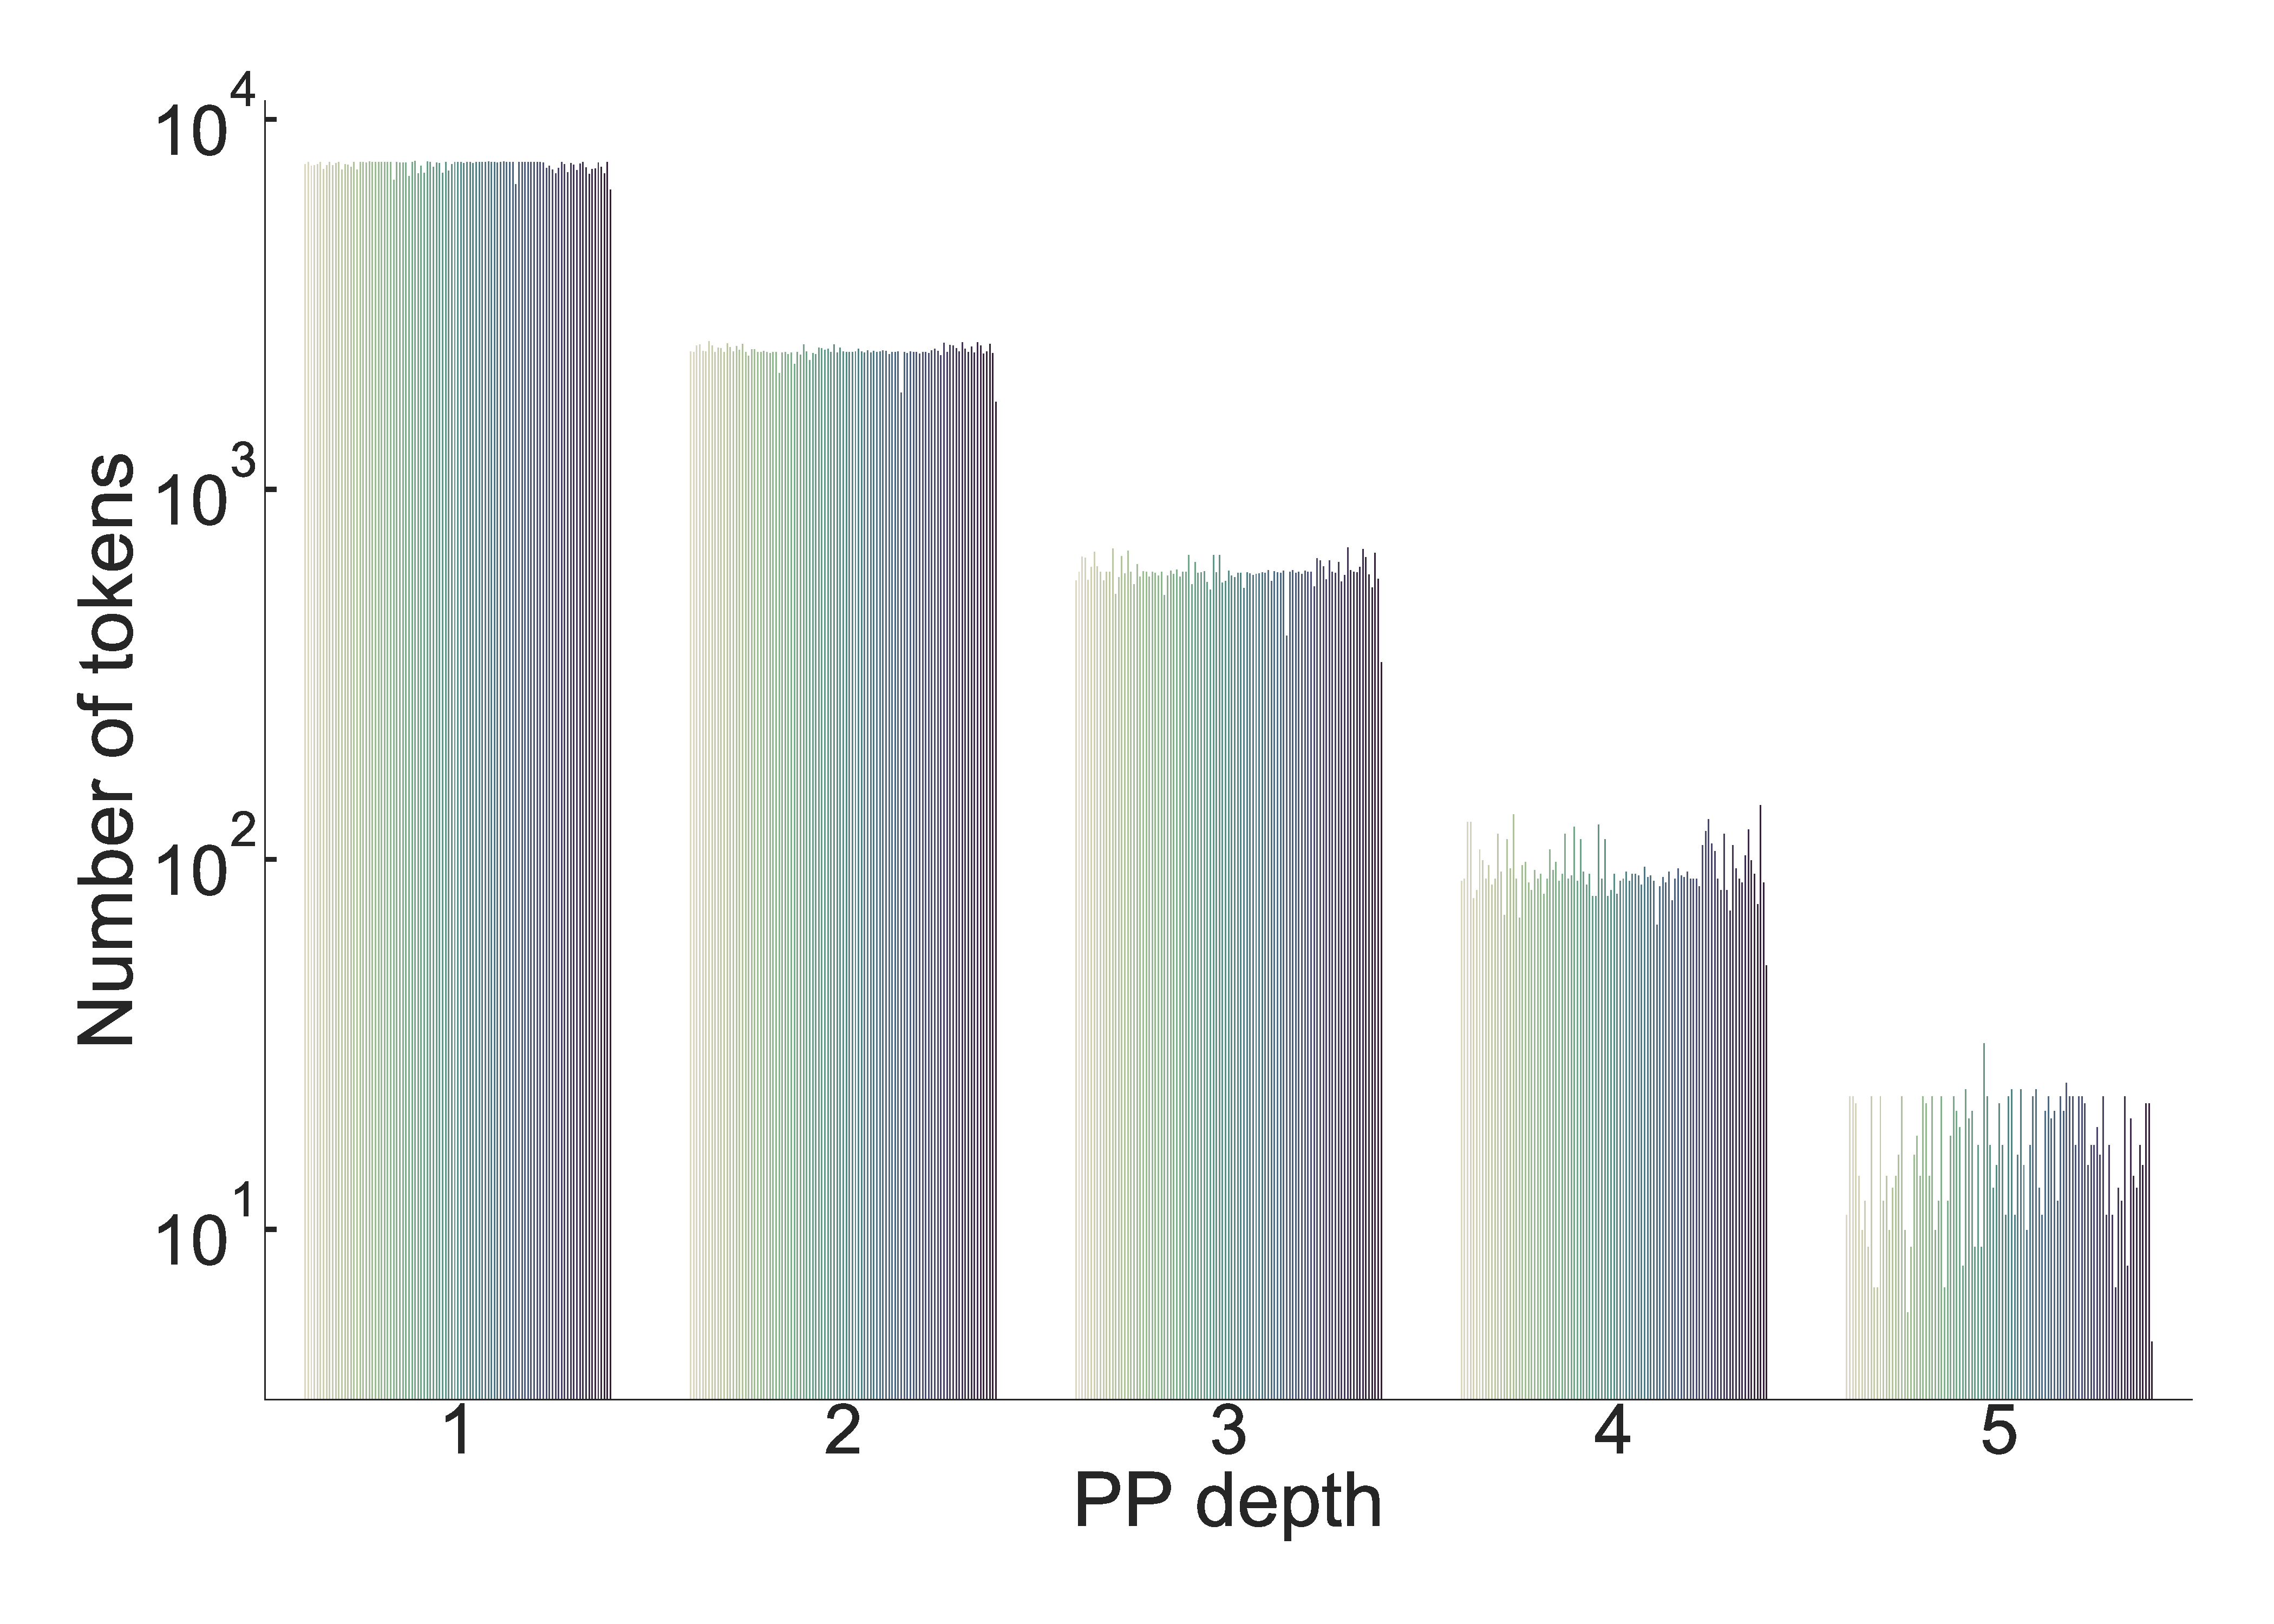
\includegraphics[width=\columnwidth]{figs/pp_depths.pdf} \end{figure*}

%\begin{figure*} \centering \includegraphics[width=\columnwidth]{figs/ttr_curve_nolegend.pdf} \end{figure*}

%\begin{figure*} \centering 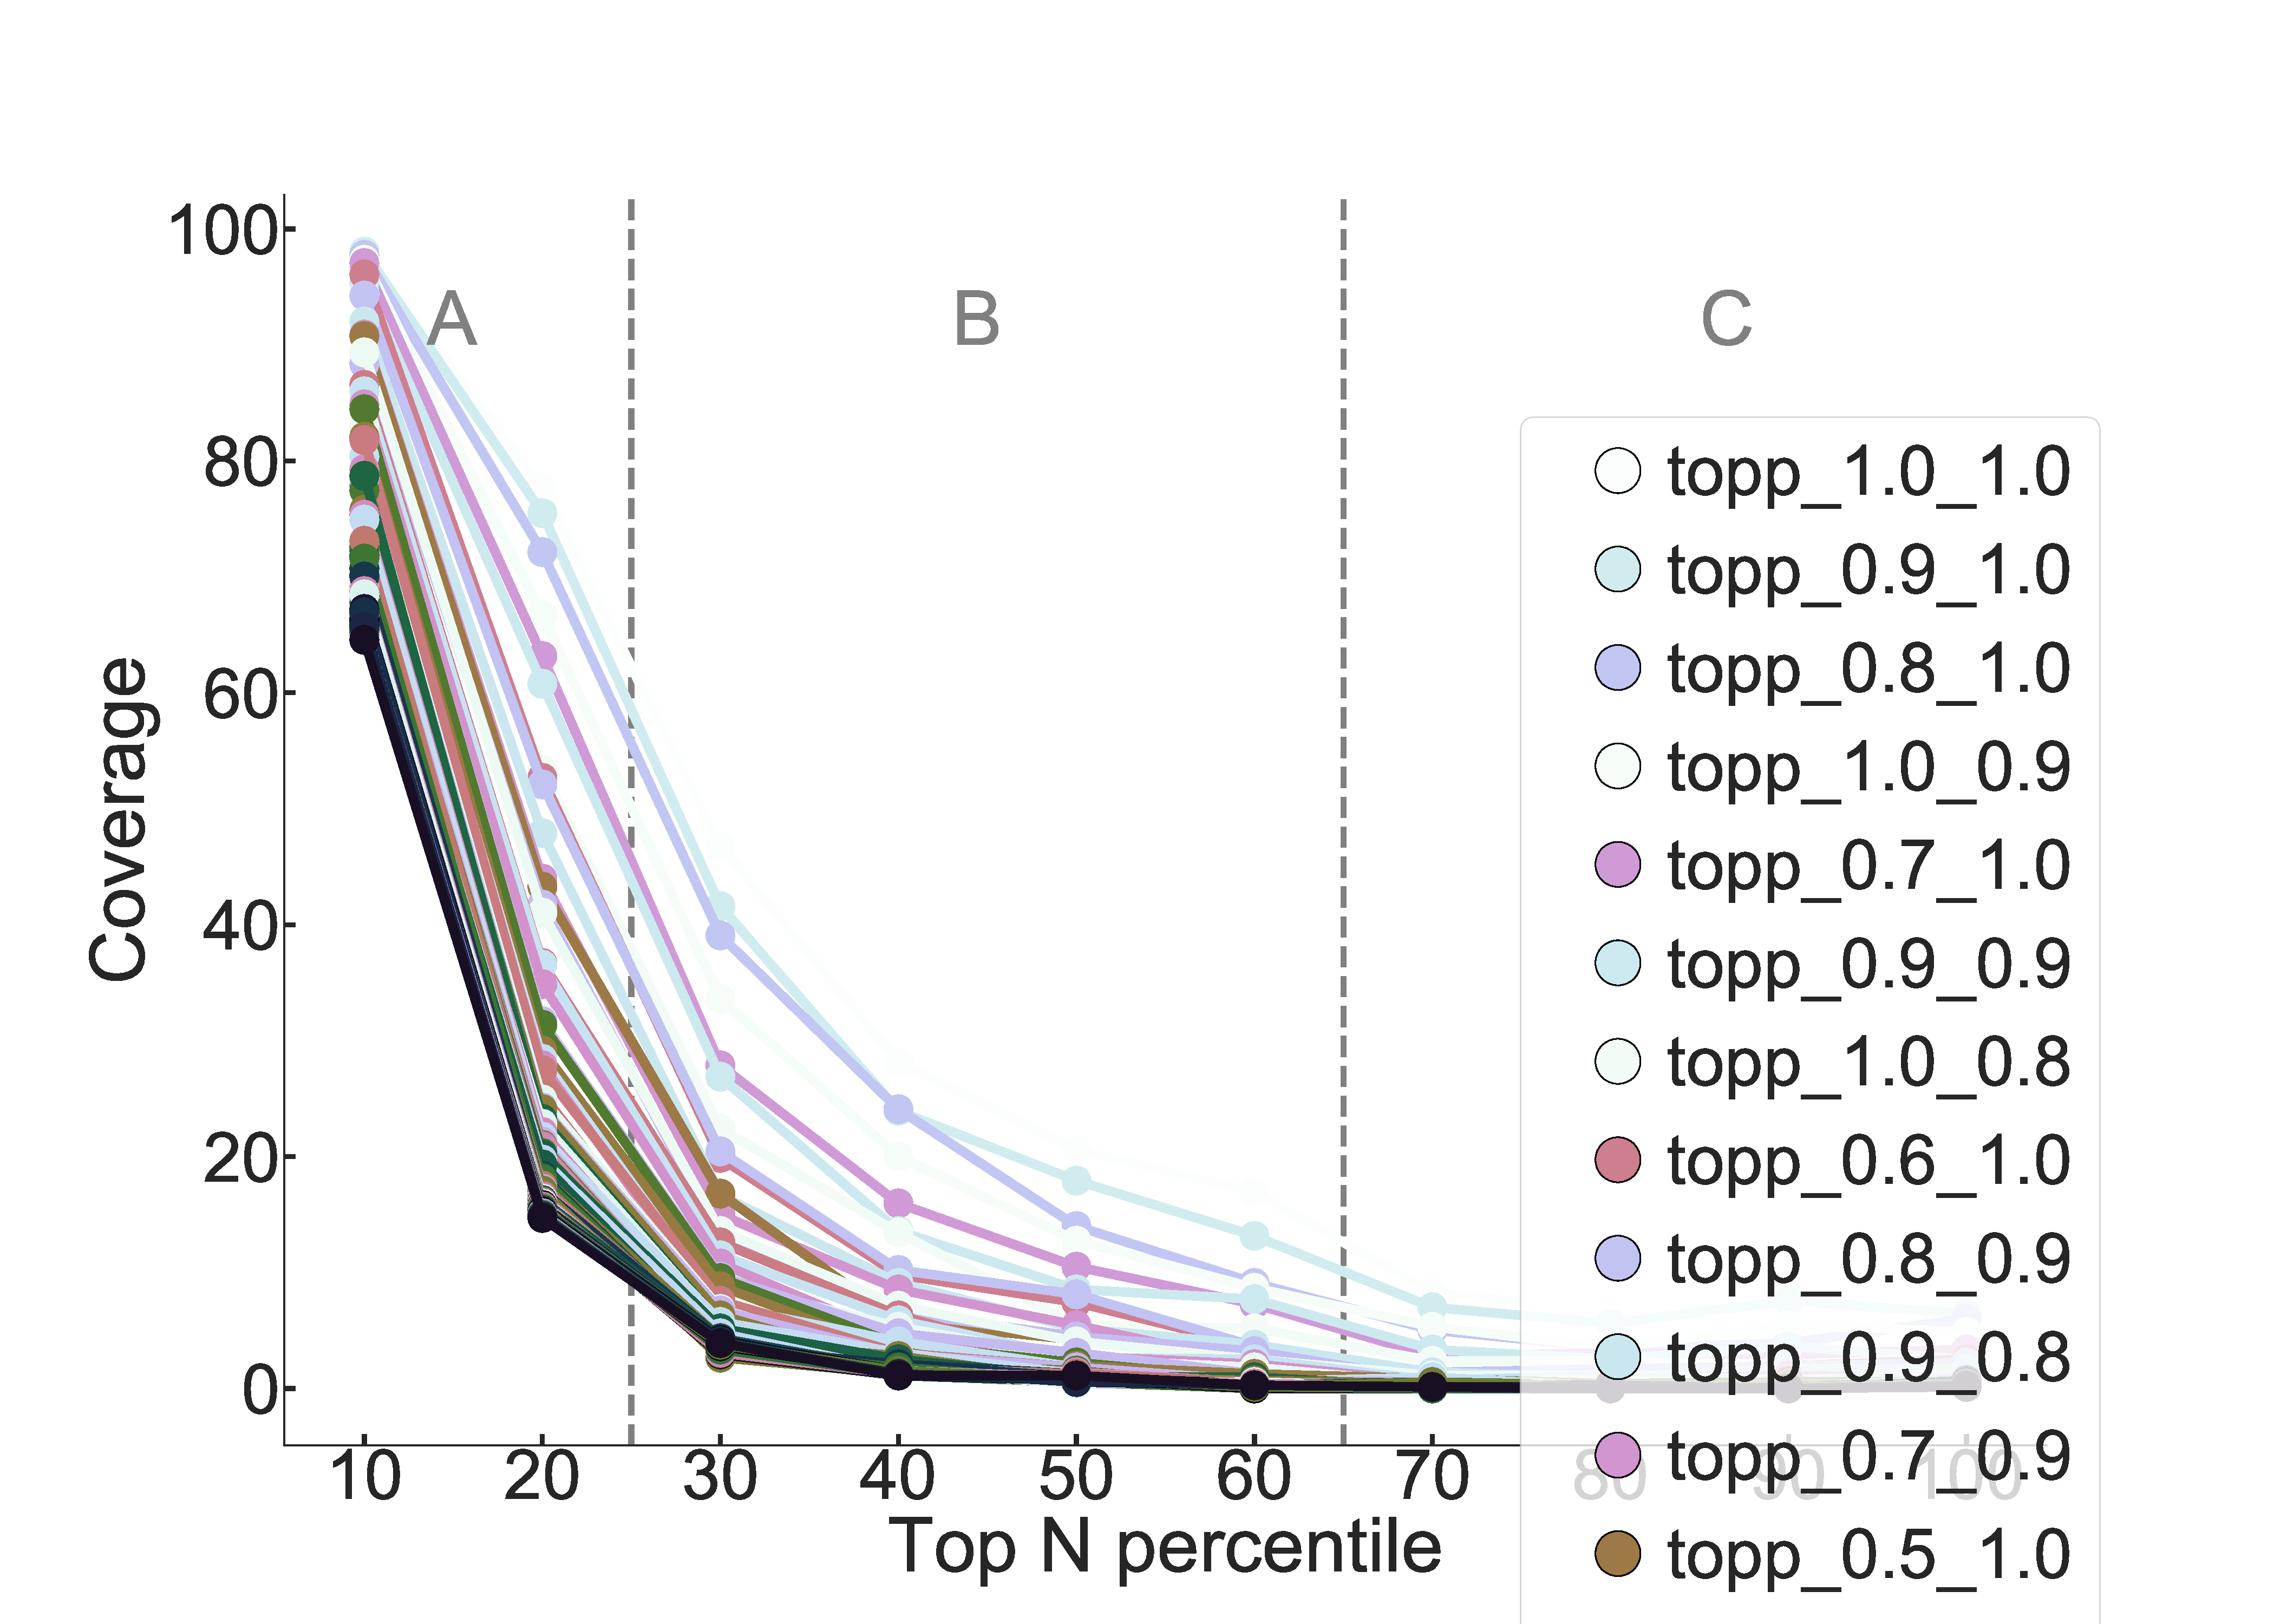
\includegraphics[width=\columnwidth]{figs/percentiles.pdf} \end{figure*}

%\begin{figure*} \centering 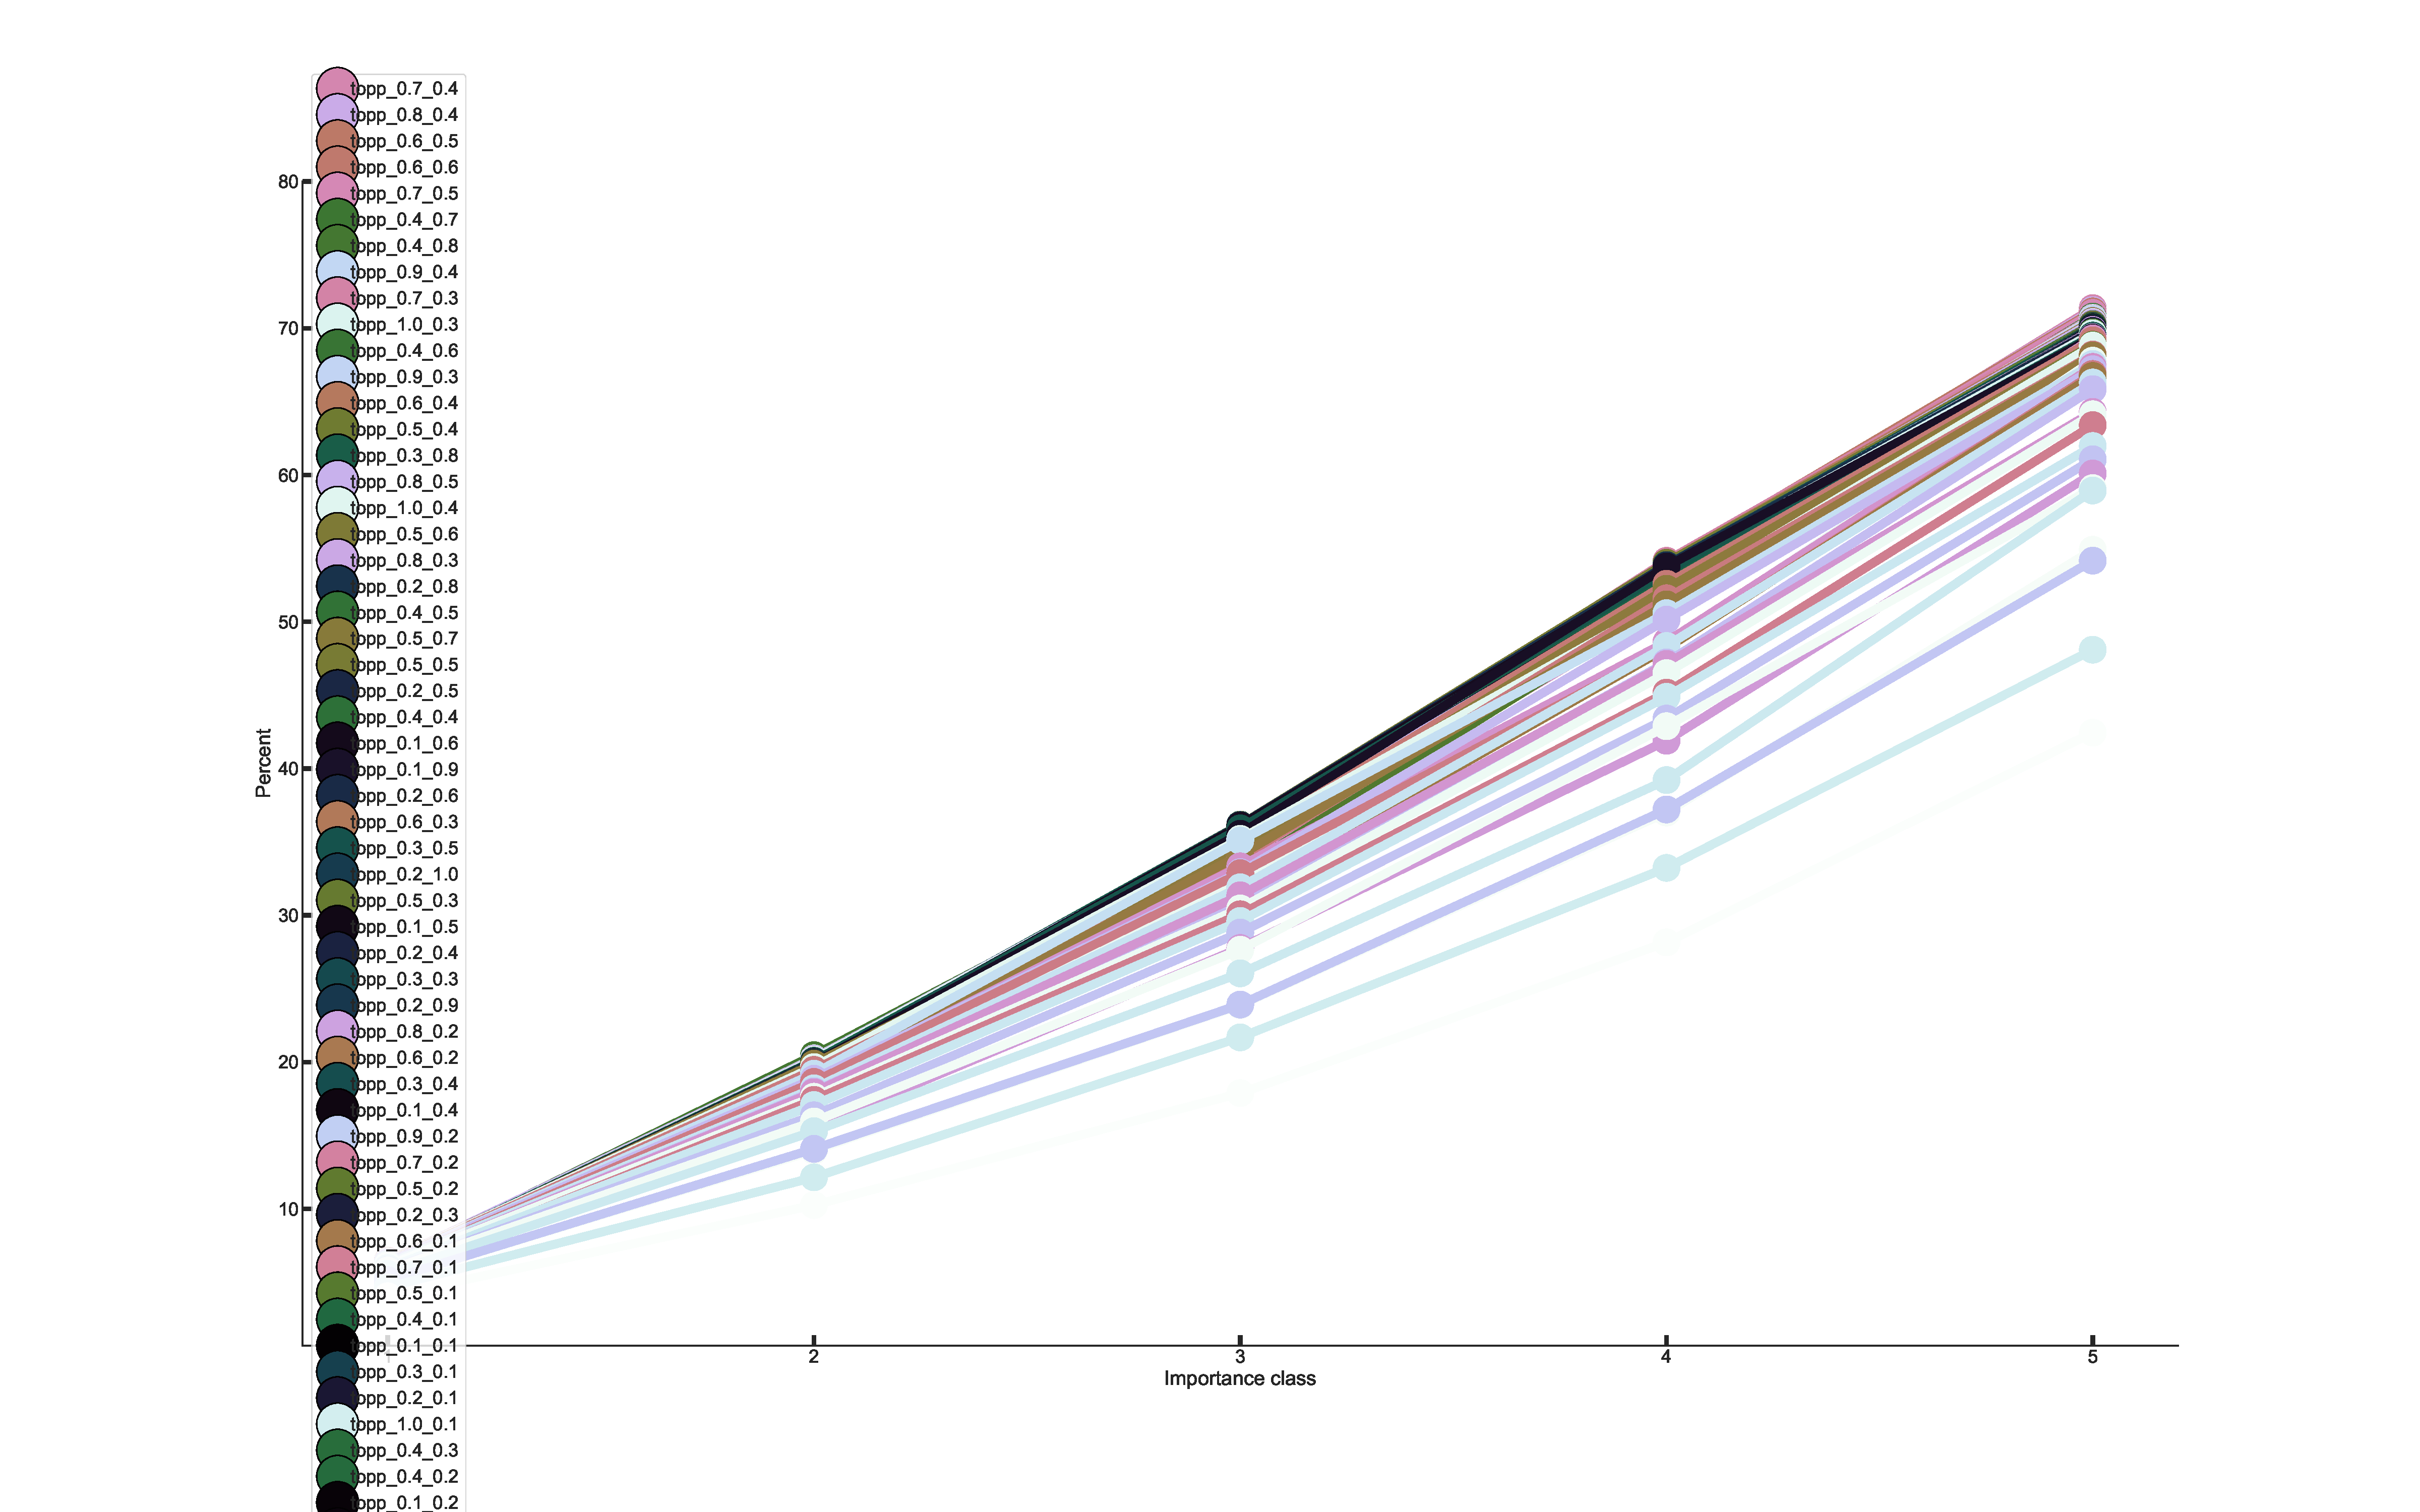
\includegraphics[width=\columnwidth]{figs/local_recall.pdf} \end{figure*}

%\begin{figure*} \centering 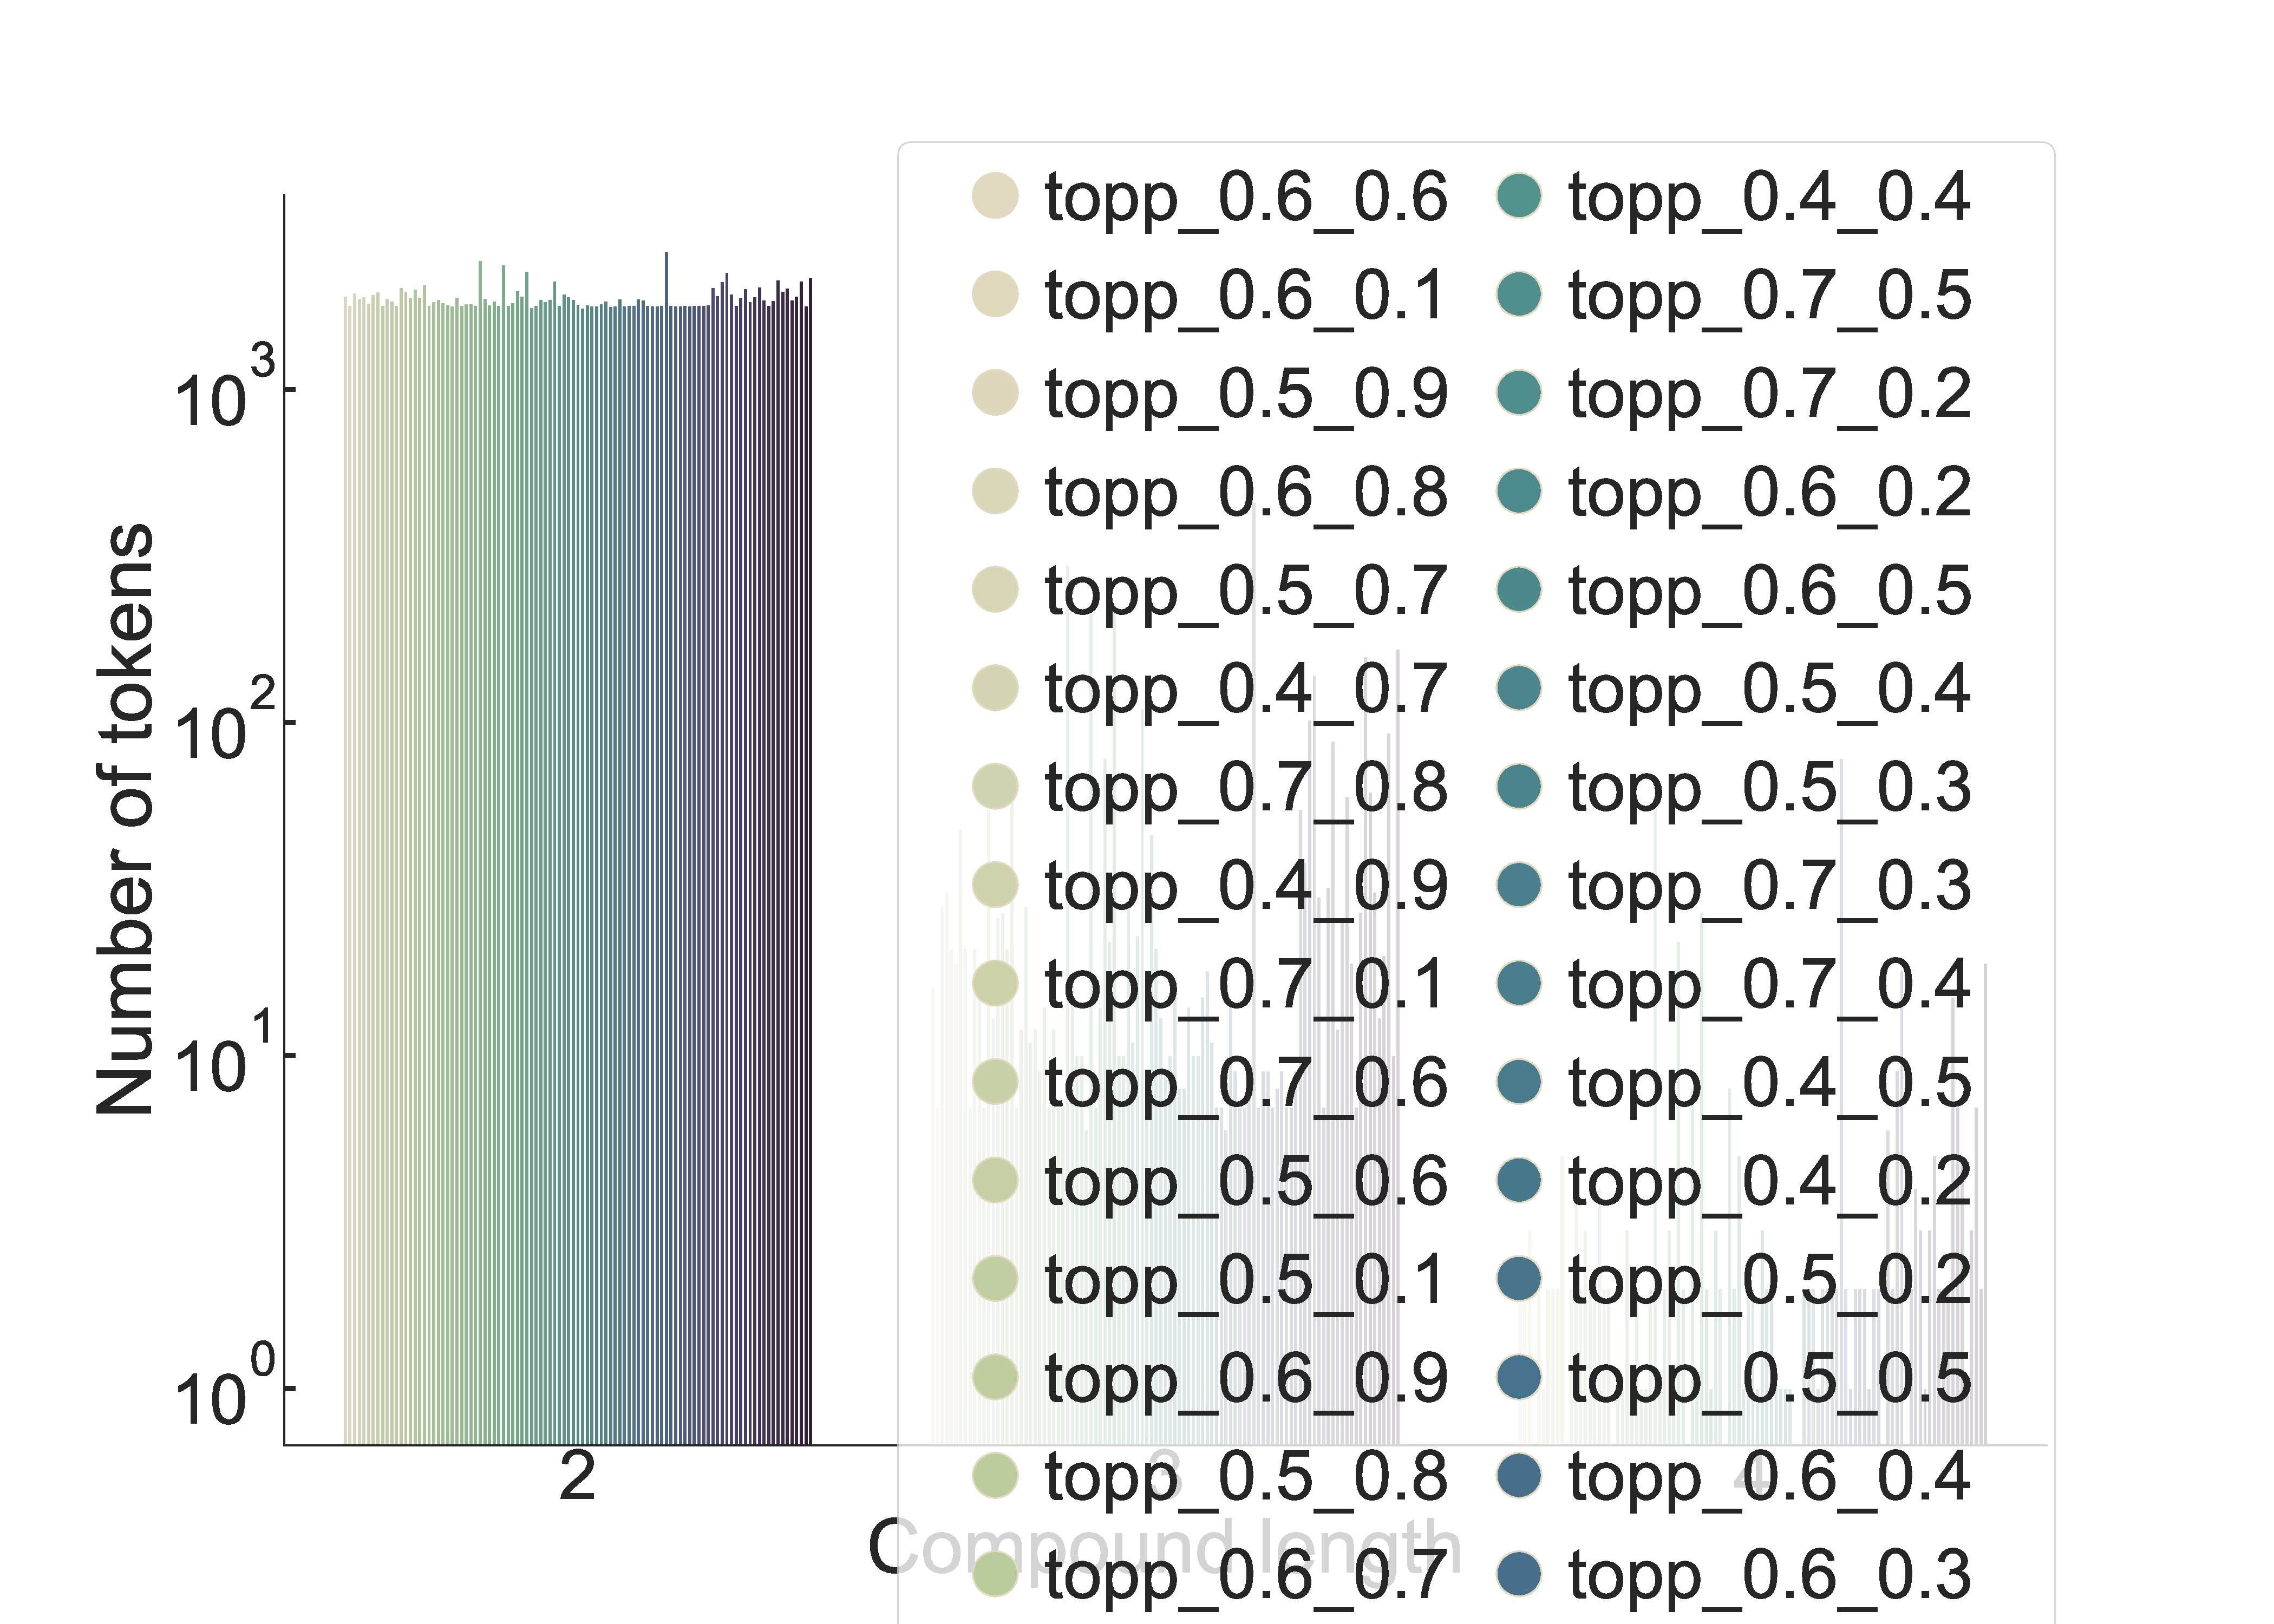
\includegraphics[width=\columnwidth]{figs/compound_lengths.pdf} \end{figure*}

\subsection{Vocabulary}

\begin{table*}
\centering
\small
\begin{tabular}{lllrrrrrrr}
\toprule
{} & {} & \multicolumn{2}{c}{\% OOV} & \multicolumn{2}{c}{freq} & \multicolumn{2}{c}{gained} & \multicolumn{2}{c}{lost} \\
{\# Dist.} & {Decoding} &  tokens &  types &  tokens &  types &  tokens &  types &  tokens &  types \\
\midrule
- & greedy        &         0.046 &        3.147 &       60.823 &     622.065 &              - &             - &            - &           - \\
- & beam          &         0.010 &        0.966 &       51.799 &     447.832 &            405 &            57 &         1207 &         201 \\
- & nucleus$_{vocab}$ &         0.050 &        2.904 &       70.238 &     744.803 &            704 &           325 &           60 &          43 \\
- & nucleus$_{bleu}$  &         0.300 &       11.385 &      103.326 &    1256.423 &           2289 &           773 &           53 &          35 \\
- & nucleus$_{grid}$  &         0.030 &        2.063 &       61.734 &     696.499 &            180 &           127 &           81 &          64 \\
3 & RSA$_{r0.5}$       &         0.027 &        1.926 &       64.447 &     648.368 &            230 &           119 &           78 &          62 \\
3 & RSA$_{r1.0}$       &         0.021 &        1.724 &       65.717 &     688.081 &            262 &           129 &           67 &          56 \\
3 & RSA$_{r2.0}$       &         0.022 &        1.449 &       67.404 &     699.356 &            335 &           175 &           59 &          49 \\
3 & RSA$_{r3.5}$       &         0.030 &        1.669 &       67.476 &     667.208 &            423 &           202 &           57 &          49 \\
3 & RSA$_{r5.0}$       &         0.037 &        2.116 &       68.609 &     667.301 &            514 &           229 &           56 &          43 \\
5 & RSA$_{r5.0}$       &         0.043 &        2.740 &       70.945 &     664.586 &            565 &           265 &           41 &          38 \\
10 & RSA$_{r5.0}$      &         0.054 &        3.398 &       75.940 &     787.023 &            813 &           333 &           39 &          34 \\
\bottomrule
\end{tabular}
\caption{lexical diversity statistics for decoding strategies. Out of vocabulary words are assessed in respect to the words in the training data, type/token frequency is expressed in terms of the average rank in the training tokens sorted by frequency. gained and lost types/tokens are assessed in comparison to the greedy baseline.}
\end{table*}

\paragraph{Out-of-vocabulary words} ratio of OOV types and tokens? text or table
compared to speaker train split

\paragraph{New Types} number and frequency

\paragraph{Zipf} compared to speaker train split

\paragraph{Examples}

\begin{itemize}

\item method
	\begin{itemize}
	\item out of vocabulary words generated (with respect to the training captions)
	\item more in-depth analysis of the vocabulary generated by the decoding strategies
	\item types gained / lost in comparison to greedy decoding (or other decoding strategies)
	%\item display of the word types generated

	\item average word frequency (with respect to the training captions)
	\item zipf (coefficient / visual?)
	\end{itemize}

\item goal
	\begin{itemize}
	\item determine more detailed differences between decoding strategies (not only TTR, novel captions or numbers of types generated)
	\end{itemize}

\item results
	\begin{itemize}
	\item
	\end{itemize}

\end{itemize}


\section{General Discussion}

\begin{itemize}

\item rsa decoding appears to lead to increased lexical diversity. that confirms our hypothesis, that context and pragmatic constraints cause lexical diversity, in NLG as well as in human language

    \begin{itemize}
        \item promising directions: trainable decoding? combining decoding strategies, if compatible?
        \item unclear: how does decoding affect interpretability of attention?
    \end{itemize}

\end{itemize}

\section{Conclusion}

future work: 
\begin{itemize}
    \item word level
    \item REG task (e.g. on RefCOCO or RefCOCO+)
    \item structural diversity (does pragmatic decoding lead to different syntactical structures to be produced?)
\end{itemize}


% Bibliography
target image against a set of similardistractor images (method adopted fromCohn-Gordon et al.)–accuracy or MRR of decisions used tocompare the models•goal–check success of pragmatic decoding–determine whether the increased linguis-tic diversity in nucleus decoding is usedpurposefully–see how the non-RSA decoding strate-gies compare to RSA decoding and toeach other
\bibliographystyle{acl_natbib}
\bibliography{anthology,emnlp2020,literature}

%\appendix

%\section{Appendices}

\end{document}
